\chapter{Artigo 02: A Python/Zig optimized and customizable
implementation for \pdcca~and \dmc~coefficients}
\label{cap:paper_02}

\begin{flushright}
    ``Just remember, \\
    once you're over the hill\\
    you begin to pick up speed.''\\[10px]
    (Charles M. Schulz)
    \end{flushright}


O artigo \emph{A Python/Zig optimized and customizable
implementation for \pdcca~and \dmc~coefficients} está sendo revisado com o objetivo de ser publicado na revista \emph{Journal of Statistical Software}. Apresenta um pacote \emph{Python} com métodos de cálculo das funções \dfa~e \dcca e dos coeficientes \pdcca~e \dmc. Os cálculos mais custosos foram implementados em programação de nível mais baixo, utilizando uma linguagem de sistemas, nova e promissora, chamada \emph{Zig}~\url{https://ziglang.org/}. A escolha da linguagem \emph{Zig}~se deu por vários motivos: 

\begin{itemize}
\item Por ser uma linguagem de baixo nível, obtendo velocidades de processamento compatíveis com \emph{C} e \emph{Fortran}~\cite{10820804, Kacs_2024}.
\item Possui compatibilidade com \emph{C} e \emph{C++}, podendo incorporar bibliotecas.
\item Possui uma sintaxe moderna e elegante para tratar problemas de baixo nível.
\item Tem um eficiente sistema de \emph{cross-compilation}.
\end{itemize}

O aspecto das \emph{cross-compilation} foi um dos mais considerados na escolha da linguagem. A manutenção de uma biblioteca por um pequeno grupo de pessoas possui diversos desafios. A capacidade de fornecer programas compilados para diversos sistemas operacionais e arquiteturas de processadores é uma etapa crucial para a popularização de um pacote. A possibilidade de se gerar os executáveis desta biblioteca em um único computador pessoal pareceu uma opção vantajosa.

\begin{algorithm} \caption{Detrended Saved} \label{alg:det_reused}
  \begin{enumerate}[label=4.\alph*]
      \item \textbf{Calculando o \emph{Detrended Value}}: Para cada série $X^{j}$ (incluindo a variável dependente) onde  $1 \ge j \ge m$, sendo $m$ o número de séries temporais; para cada escala temporal, em cada caixa $i$, calcula-se o valor de $DV^{j}_{k,i} = (X^{j}_{k,i}-\widetilde{X^{j}}_{k, i})$ e armazena-se em uma matriz. A matrix tem por dimensões $m, n+1$, onde cada linha corresponde a uma série temporal e as colunas correspondem ao número de pontos em cada caixa.
      \item \textbf{Cálculo da função $f_{DFA}^{2}$ para cada caixa}: Calcula-se o valor do \dfa~:\\[10pt]
          $f_{DFA}^{2}(n, i) = \frac{1}{1+n} \sum_{k=i}^{i + n}(DV^{j1}_{k,i})^{2}$;
      \item \textbf{Cálculo da função $f_{DCCA}^{2}$~em cada caixa}: com a matriz $DV$ devidamente preenchida, para uma das $N - n$ caixas de uma mesma escala temporal a função é calculada para todas as combinações de séries temporais duas à duas por:\\[10pt]
          $f_{DCCA}^{2}(n, i) = \frac{1}{1+n} \sum_{k=i}^{i + n}(DV^{j1}_{k,i}) \times (DV^{j2}_{k,i})$
      \item \textbf{Retomando o algorítimo padrão}: Após o cálculo de todas as caixas, aplica-se o passo 5 do \dfa~e \dcca. 
  \end{enumerate}
  \end{algorithm}

O \emph{software} de cálculo de dinâmica de fluidos computacional \emph{AeroSim}~\url{https://aerosim.io/} apresenta desempenho e precisão nos seus cálculos \cite{romanusViableFrameworkWind2023, lugariniLargeEddySimulations2024} é parcialmente implementado em \emph{Zig} e serviu de incentivo à esta adoção.

Parte da otimização segue a implementação de \citeonline{hartmannRealtimeFractalSignal2013} para o \dfa, transposta para o \dcca~e \pdcca~por~\citeonline{Kapostza2022}. Onde, durante o cálculo da interpolação da reta de tendência, na primeira caixa de cada séries, pelo método dos mínimos quadrados, valores são gravados em variáveis que podem tornar o \emph{loop} de somatórios dos valores utilizados no cálculo dos coeficientes da equação da reta são armazenados em variáveis. Para a caixa seguinte, o \emph{loop} é substituído por operações de subtração e adição.



A Equação~\ref{eq:sum_opt_x}, mostra que o valor da soma das coordenadas no eixo das abscissas de uma caixa pode ser substituído pelo somatório total na caixa anterior menos o primeiro valor de abscissa da caixa anterior, somado ao último valor de $x$ para a caixa atual. Raciocínio análogo pode ser aplicado às Equações~\ref{eq:sum_opt_x2}, \ref{eq:sum_opt_y}~e~\ref{eq:sum_opt_xy}.

\begin{equation}
    \label{eq:sum_opt_x}
    \forall~1<i\leq(N-n),~\sum_{k=i}^{i + n}T_k = \left(\sum_{j=i-1}^{(i+n)-1}T_j\right)~-~T_{i-1}~+~T_{i + n}
  \end{equation}
  
  \begin{equation}
    \label{eq:sum_opt_x2}
    \forall~1<i\leq(N-n),~\sum_{k=i}^{i + n}T_k^2 = \left(\sum_{j=i-1}^{(i+n)-1}T_j^2\right)~-~T_{i-1}^2~+~T_{i + n}^2
  \end{equation}
  
  \begin{equation}
    \label{eq:sum_opt_y}
    \forall~1<i\leq(N-n),~\sum_{k=i}^{i + n}S_k = \left(\sum_{j=i-1}^{(i+n)-1}S_j\right)~-~S_{i-1}~+~S_{i + n}
  \end{equation}
  
  \begin{equation}
    \label{eq:sum_opt_xy}
    \forall~1<i\leq(N-n),~\sum_{k=i}^{i + n} (S_k\times T_k) = \left(\sum_{j=i-1}^{(i+n)-1}(S_j \times T_j)\right)-(S_{i-1} \times T_{i-1})+(S_{i + n} \times T_{i + n})
  \end{equation}

Quando se pensa no cálculo do \dmc, e em como otimiza-lo, deve-se pensar em múltiplos cálculos de \pdcca, para a criação da matriz apresentada na Equação~\ref{eq:p_dcca_matrix}. A ideia é substituir o passo 4 do Algoritmo~\ref{alg:dcca} pelos passos descritos no Algoritmo~\ref{alg:det_reused}.



Essa pequena mudança, embora possa até aumentar o tempo de processamento para um pequeno número de séries temporais, demonstra-se muito vantajoso quanto maior for o número de séries cujo coeficiente \pdcca~ precisa ser calculado.

\begin{equation}\label{eq:combinations_2x2}
  \frac{j!}{2 \times (j-2)!}
\end{equation}

Na biblioteca \emph{Zebende} é possível implementar outras versões do código para o cálculo do \pdcca~com poucas séries temporais. Mas é preciso entender em que ponto o Algoritmo~\ref{alg:det_reuse} passa a ser vantajoso. Caso o $DV$ não seja armazenado, o número de vezes que ele tem que ser calculado é de duas vezes o número de combinações duas a duas para $j$ séries~(Equação~\ref{eq:combinations_2x2}) e o tempo gasto para calcular o $DV$ depende do tamanho das séries.

Vale também ressaltar que as otimizações baseadas no salvamento dos parâmetros do método dos mínimos quadrados pode ser adaptado para diversos graus do polinômio da tendência, mas não pode se adaptar à caixas não sobrepostas.

Como apresentado na Sessão\ref{ss:dfa_fract} do Capítulo~\ref{cap:fund_teorica}, alguns autores ainda advogam pela não sobreposição das caixas~\cite{zhouMultifractalDetrendedCrosscorrelation2008}, nestes casos, o armazenamento dos parâmetros para o cálculo dos mínimos quadrados não funcionaria. Por outro lado, para uma grande quantidade de séries temporais o Algorítimo~\ref{alg:det_reused}, \emph{Detrended Saved}, funcionaria também no cenário de caixas não sobrepostas.

Além da otimização, o artigo apresenta o modo de uso da biblioteca e algumas das funções auxiliares já implementadas. As equações destacadas nas Sessões~\ref{ss:dfa_fract}~e~\ref{ss:vari_cross} do Capítulo~\ref{cap:fund_teorica} estão entre as próximas adições ao pacote.

O código fonte da biblioteca \emph{Zebende} está disponível em \url{https://github.com/255ribeiro/zebende}.


    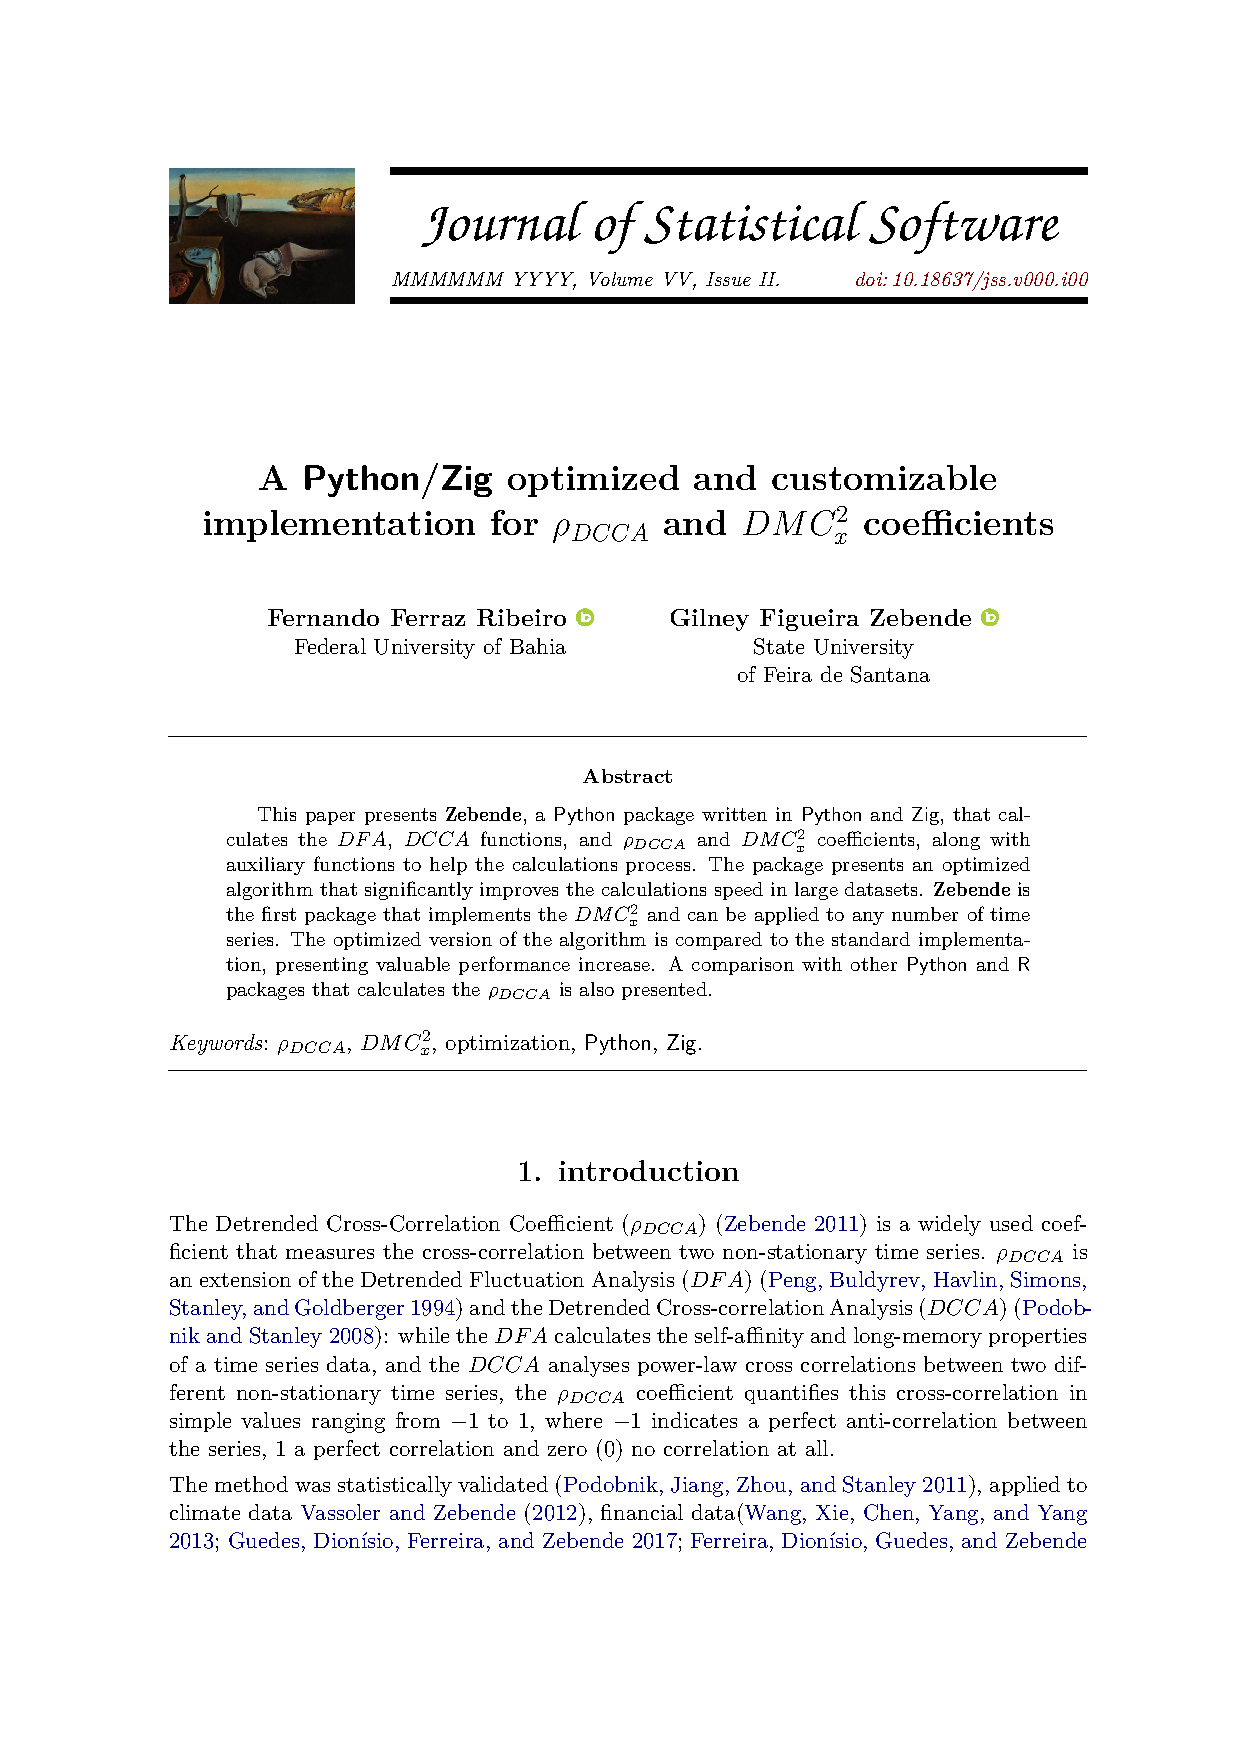
\includepdf[pages=-, pagecommand={\thispagestyle{plain}}]{./Papers_publi/paper_zebendelib.pdf}